%\documentclass[12pt]{report}
%\usepackage{kjfsty}
%
%\begin{document}
%
%\tableofcontents
%\onehalfspacing

%\renewcommand{\sfdefault}{phv}
%\renewcommand{\rmdefault}{ptm}
%\renewcommand{\ttdefault}{pcr}


\setcounter{chapter}{0}
\chapter[Introduction]{Introduction}
%\addcontentsline{toc}{chapter}{Introduction}
%\chaptermark{Introduction}
%\markboth{Introduction}{Introduction}

Never a dull moment.  Not in the field of optoelectronics; not since %its creation some half century ago with the merging of semiconductors and optics. where
the merging of semiconductors and optics was cemented some half century ago after Chapin and colleagues at Bell Labs made practical use of the photovoltaic effect in a silicon solar cell \cite{Chapin:JAP:1954}.  And of the many defining moments in optoelectronics research, perhaps paramount of them all was the first observations in 1962 by Hall \emph{et al.} \cite{Hall:PRL:1962} and Holonyak \emph{et al.} \cite{Holonyak:APL:1962} of stimulated emission in electrically pumped semiconductors.  Since that time, optoelectronic technology has become an integral part of our daily lives.  Solar cells may well be on the verge of contributing to the elimination of fossil fuels.  Light emitting diodes (LEDs) are rapidly replacing Edison's incandescent bulb.  How many liquid crystal display (LCD) devices do you own... too many to count in a single attempt?

Semiconductor laser technology is no different.  Without these lasers, our telecommunications pipelines would be vastly less efficient.  We would be relying on the same technology that powered Henry's electromagnetic telegraph: electrons traveling through wire (slow) rather than photons traveling through glass (fast!).  Today's semiconductor lasers, and indeed to varying degrees most all optoelectronic devices,  make use of a fundamental concept dubbed heterostructure engineering.  In fact, the heterostructure's ubiquity was recognized by the year 2000 Nobel prize in physics, awarded to Zhores Alferov \cite{Alferov:NobelLecture} and Herbert Kr\"omer \cite{Kroemer:NobelLecture} for their pioneering work.  A heterostructure device is composed of layers of different materials, overlayed one after the other.  These layers are strategically selected and used to precisely control how electrons---\emph{i.e.} current---pass through a device.

The layers that make up a heterostructure can be made exceedingly thin: thicknesses on the order of a single atomic layer.  The ability to form such thin layers make heterostructures one of man's ultimate engineering conquests of quantum mechanics.  Just as nature's atom puts electrons into discrete energy orbits, man's quantum-confined heterostructure forces electrons into discrete energy states as they pass through a heterostructure device.  By exploiting this ability, we can influence when, where, and how electrons interact with their surroundings.  In the seminal work that first recognized this possibility of quantum confinement in heterostructures, Esaki and Tsu in 1970 theorized that a particular heterostructure implementation could result in \emph{negative} resistance at certain applied voltage levels \cite{EsakiTsu:IBM:1970}.  The following year, Kazarinov and Suris proposed that the man-made energy states of quantum-confined heterostructures could be used as the basic optical transition for a new type of laser \cite{KazarinovSuris}.  Despite multiple attempts, it took some 25 years to realize such an intersubband heterostructure laser \cite{Faist:Science:1994}, now known as the quantum cascade (QC) laser.  The year 2009 marks the 15th anniversary of the first reported QC laser demonstration.

The genius of the heterostructure concept---and the quantum cascade in particular---lies in its innate engineerability.  In this thesis, I hope to convey how the QC concept provides vast opportunity for creative new ideas that can expand technological capabilities and improve device performance.

%it leaves unbounded the limits of what is possible to make.  This thesis explores several examples

%The quantum cascade is a synthetic structure, wholly man-made

%This thesis explores novel and innovative new ways of producing mid-infrared light.

%We can create artifical materials, or materials with properties that are completely man-made, not existing in nature.


%Intersubband devices give engineers a degree of versatility that is flat out unprecedented  in active optoelectronic devices.  What makes intersubband devices in general, and QC lasers in particular, so damn configurable and customizable?
%It's a knob that is on its face elementary to turn.  We don't have to fight with nature, to coerce it into something it doesn't want to do.  Like what happens with much of today's technology.

%QC lasers are fun.  There's a low barrier to entry.  A first year graduate student can grow a functioning laser in the first shot.  It wasn't a good laser; I made the mistake of doping the entire injector region, when only a few select wells should have been doped.  But the point is, it worked.  Making a working laser is easy.  Making a good laser is much more difficult.

%The system does have its challenges, limitations to the current state-of-the-art.


\section{Engineered Mid-infrared Light Sources: Present and Future}
%\addcontentsline{toc}{section}{Quantum Cascade Lasers}

QC lasers are particularly suited for generating light at mid-infrared (mid-IR) wavelengths.  Loosely defined, the mid-infrared is the spectral region between 3 and 30~\um\ in wavelength (10--100 THz in frequency).  As illustrated in Fig.~\ref{intro:rgbir}, these boundaries mark convenient transitions between the capabilities of three different technologies that are today's most capable electrically-pumped semiconductor-based laser sources.  From the visible region to about 3~\um\, diode lasers dominate \cite{Alferov:NobelLecture} \cite{Kroemer:NobelLecture}; diode lasers are especially capable at the 0.98 and 1.55~\um\ ``telecom'' bands.  On the long wavelength side, THz QC lasers are the dominant injection laser technology  \cite{Williams:NatPhot:2007:THzReview}.  Although Pb-salt diode lasers were once the best option for mid-infrared injection sources, QC lasers have emerged as far more capable devices. Mid-infrared QC lasers span 2.75~\um\ \cite{Devenson:APL:2007} to 24~\um \cite{Colombelli:APL:2001:24um}, with various performance levels in between.  In general, room temperature (RT), continuous wave (CW) lasing is now the technological standard from 4--12~\um.  %Today's wall-plug efficiency record is 65\% at low temperatures.  Mid-IR qc lasers, the field is advancing most rapidly, of the three technologies.

%Diode lasers are a mature technology.  No fundamentally new and highly impactful advances have been made for some time.  The understanding is almost complete.  We've gotten everything we can get out of them.

%THz, in terms of capabilities, is still relatively nascent.

%Mid-IR QC lasers are somewhere between.  While they are relatively mature in terms of capaibilities, the performance is still rapidly improving.


\begin{figure}[tp]
\centering
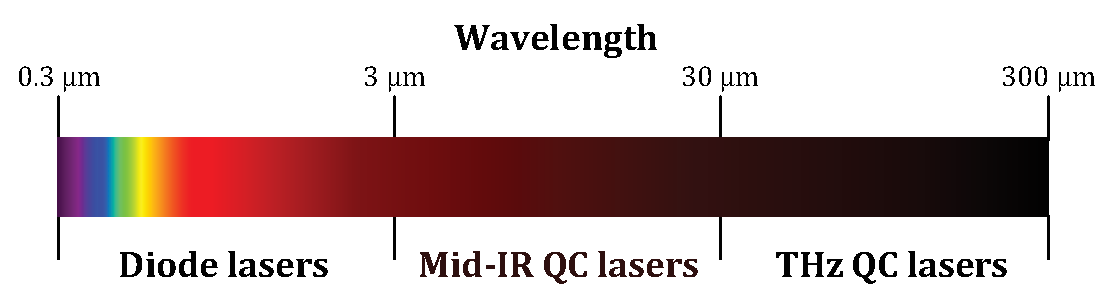
\includegraphics[width=6in]{introduction/rgbir_spectra}
\caption[The electromagnetic spectrum]{\tn{\textbf{The electromagnetic spectrum.}}  The wavelengths from $0.3$ to $300~\tn{\um}$ are covered by three semiconductor laser technologies.  The mid-infrared, loosely defined as $3$ to $30~\tn{\um}$, is the regime of mid-infrared QC lasers.  Between the transitions for laser device types---diode--to--mid-IR QC laser and mid-IR QC laser--to--THz QC laser---lie spectral gaps of substantial technical challenge.  The first gap, explored in Chapter~3, results from fundamental loss mechanisms in diode lasers and band offset limitations in mid-IR QC lasers.  The second gap, explored in Chapter~4, derives fundamentally from the semiconductor restrahlen band in the 30--60~\um\ region.}
\label{intro:rgbir}
\end{figure}

An ability to easily generate mid-infrared light is most certainly of technological importance.  Holding a wide swath of the electromagnetic spectrum, mid-infrared light can be exploited for unique applications.  While there are numerous applications for mid-infrared light, with more surely on the horizon, here I briefly discuss just three examples: defense countermeasures, open atmosphere data transmission, and molecular species detection.


\subsection{Defense countermeasures}
\begin{figure}[tp]
\centering
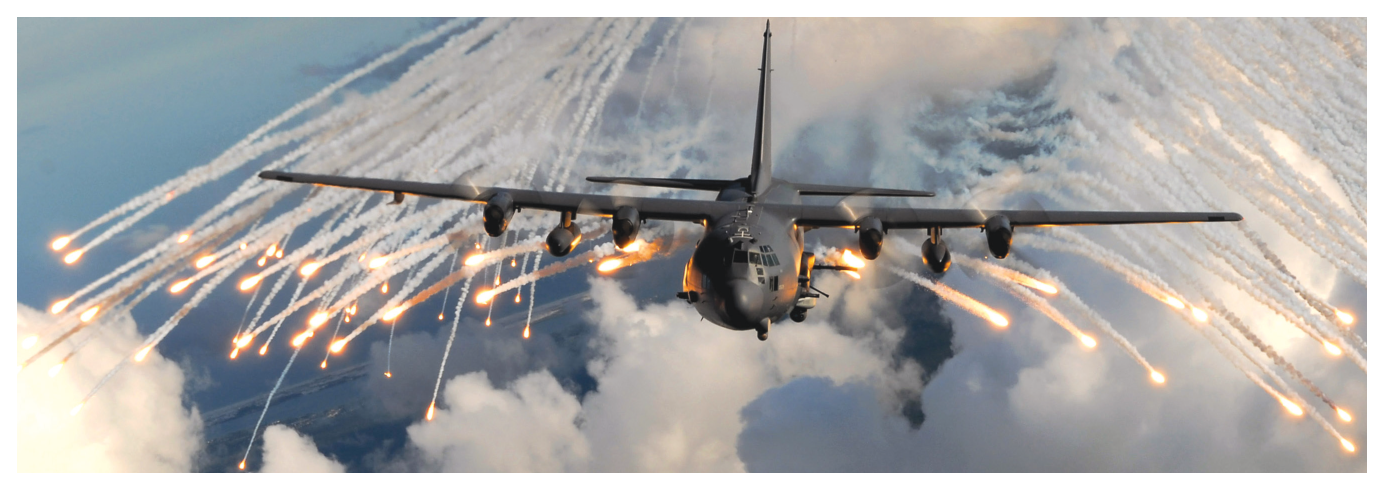
\includegraphics[width=6in]{introduction/flares}
\caption[Infrared countermeasure flares deployed from an AC-130U gunship]{\tn{\textbf{Infrared countermeasure flares deployed from an AC-130U gunship.}}  An AC-130U gunship jettisons flares over an area near Hurlburt Field, Florida. The flares are a decoy for heat-seeking missiles that may be fired at the aircraft. The aircraft is from the 4th Special Operations Squadron.  Courtesy of the U.S. Air Force \cite{USAF:AC130}.}
\label{intro:flares}
\end{figure}

Deployable flares, such as those being emitted from an AC-130U gunship in Fig.~\ref{intro:flares}, are the conventional countermeasure against IR-guided (heat-seeking) missiles.   Modern infrared countermeasures (IRCMs), which use directed infrared light sources to ``jam'' the targeting system on an IR-guided missile---in effect blinding the missile, have qualities that make them far more effective by comparison.  The ability to highly tailor the spectral signature and modulation properties of a light source is a key advantage over older flare-based technologies.  Modern IRCMs also do not require an aircraft to undergo ``evasive maneuvers'' to physically separate itself from dropped flares.  As a craft-mountable module, shown in Fig.~\ref{intro:atircm}, these systems couple threat identification and tracking together with targeting and jamming into a system that does not require expendable components such as flares.

\begin{figure}[tp]
\centering
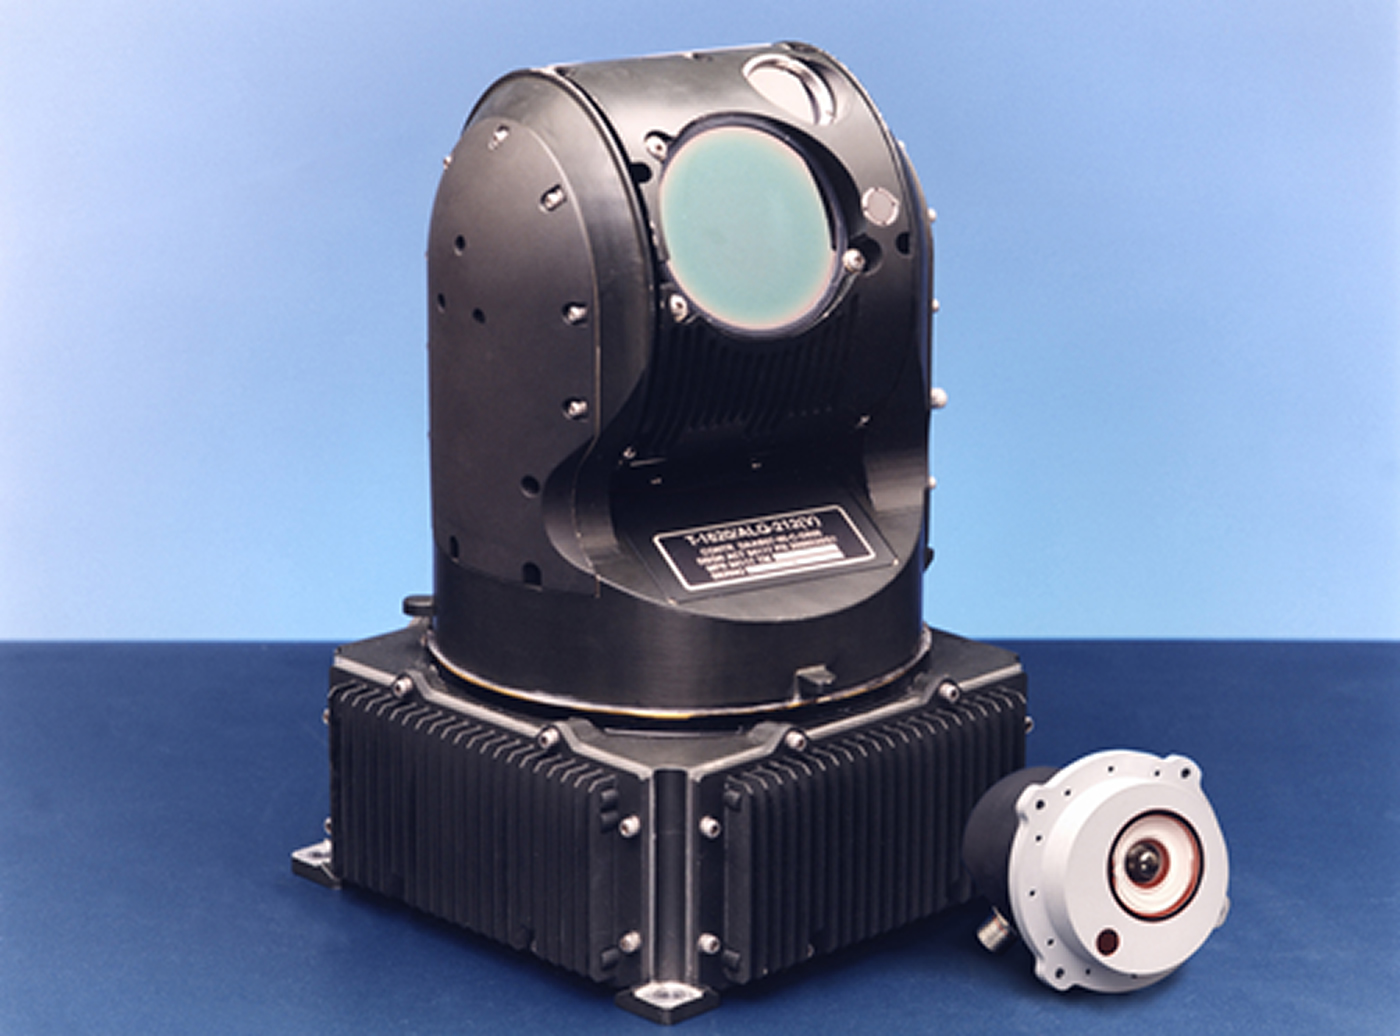
\includegraphics[height=2.25in]{introduction/atircm}
\caption[IRCM module]{\tn{\textbf{IRCM module.}}  An early photo of Lockheed Martin's ATIRCM.  Courtesy of BAE Systems press release \cite{BAE:ATIRCM}.}
\label{intro:atircm}
\end{figure}


The two modern IRCM programs, Northrup Grumman's NEMESIS Directional Infrared Countermeasure (DIRCM) and Lockheed Martin's Advanced Threat Infrared Countermeasures (ATIRCM), both use solid state laser light sources. These are bulky, only operate under pulsed conditions, and have spectral emission characteristics that are difficult to customize.  By comparison, QC lasers are miniature devices, capable of CW operation, and have spectral emission that is highly configurable.  Clearly, QC lasers are of interest to replace and improve upon the present-day IRCM light sources.

%
%The ability to generate intense, wavelength-customizable mid-infrared light


\subsection{Open atmosphere data transmission}

%also discuss lidar here

\begin{figure}[tp]%
\centering%
\subfloat[]{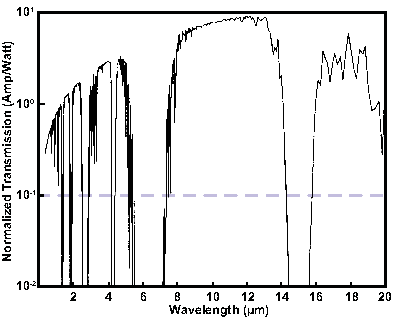
\includegraphics[width=2.795in]{introduction/atmos_a}
\label{intro:atmos_a}}%
\hfil%
\subfloat[]{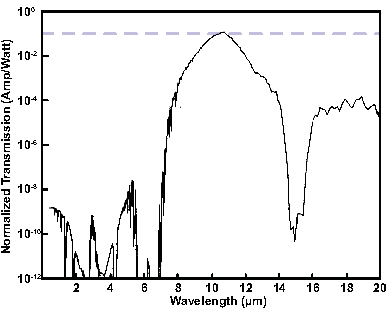
\includegraphics[width=2.8in]{introduction/atmos_b}
\label{intro:atmos_b}}%
\caption[Atmospheric absorption versus wavelength]{\tn{\textbf{Atmospheric absorption versus wavelength.}} Mid-infrared wavelengths, especially in the second atmospheric window near $10~\tn{\um}$, are considerably more ``clear'' during adverse weather. Panel \tn{(a)} shows transmission for very clear weather (``visibility,'' $50~\tn{km}$) while \tn{(b)} shows transmission for thick fog (``visibility,'' $200~\tn{m}$).  The dashed line represents normalized transmission at $10^{-1}~\tn{A/W}$ for comparison.  Reprinted from \cite{Manor:AO:2003} with permission from the Optical Society of America.}
\label{intro:atmos_trans}
\end{figure}

Methods for transmitting information through the atmosphere, and specifically free space optical communications systems, use laser-based transceivers for line-of-site data transmission. Compared to other communications technologies, free space optical communications combines capabilities of extremely high bandwidth, rapid deployment time, and license- and tariff-free bandwidth allocation.  The major weakness of free space optical communications is the threat of sporadic downtime associated with adverse weather conditions such as fog, haze, or rain that prevent the signal (light) from propagating through the atmosphere.  The wavelength-dependence of atmospheric absorption for clear and foggy conditions is shown in Fig.~\ref{intro:atmos_trans}, as calculated by Manor and Arnon \cite{Manor:AO:2003}.  For clear weather, the advanced capabilities of telecom lasers around 1.5~\um\ would certainly suffice.  Yet under adverse conditions, as shown in Fig.~\ref{intro:atmos_b}, transmission near 1.5~\um\ decreases by approximately 9 orders of magnitude.  In comparison, transmission for 10~\um\ light only decreases by 2 orders of magnitude between the two atmospheric conditions, and the difference between 1.5~\um\ light on a clear day and 10~\um\ light on a foggy day is only 1 order of magnitude.
The mid-infrared is a most convenient wavelength for applications where atmospheric transmission is important, free space optical communications included.


\subsection{Molecular species detection}

Perhaps the most versatile of the applications for mid-infrared light is its use in the detection of trace molecules.  Molecular detection based on sensing the presence of light absorption can be versatile, selective, and sensitive \cite{Kosterev:APB:2002:15um}.  Individual molecular species have unique energies at which they absorb light, the absorption energies corresponding to vibrational and rotational modes of the molecule.  Figure~\ref{intro:gasses_sectra} shows absorption spectra for several common and important atmospheric gasses.  These molecule-specific absorption ``fingerprints'' can be used to selectively determine the presence of a particular species, including isotropic ratios, by an absorption spectroscopy system.  Such a system typically has three components: a light source, a light-matter interaction space, and an optical detector.  For gas-phase absorption spectroscopy, the light source wavelength is tuned to correspond to an absorption line of a targeted molecular species, the light is allowed to interact with a gas sample in a cavity such as a Herriot cell, and the remaining light is collected on an optical detector.  All else being equal, maximum sensitivity is achieved when the frequency of the light source is selected to be on resonance with the strongest absorption line of the target species.  That is, the use of fundamental mode absorption resonances, most typically at mid-infrared wavelengths, will yield the most effective and sensitive detection systems.


\begin{figure}[tp]
\centering
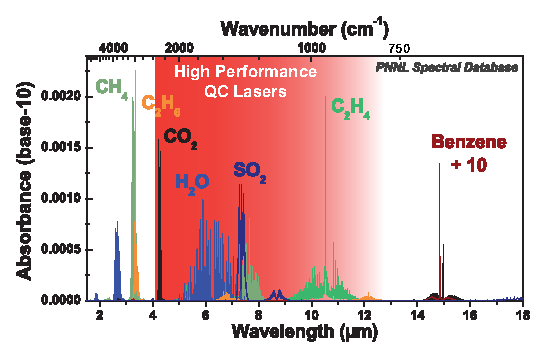
\includegraphics[width=5.25in]{introduction/benzene_ethane_methane_2}
\caption[Spectral absorption signatures for several atmospheric gasses]{\tn{\textbf{Spectral absorption signatures for several atmospheric gasses.}}  Most molecular species have their fundamental resonances at wavelengths beyond $3~\tn{\um}$, out of reach of diode lasers.  High performance (RT CW) QC lasers are able to cover a large many of the resonances of interest.}
\label{intro:gasses_sectra}
\end{figure}



\section{Quantum Cascade Lasers}

Understanding the basic operation of a QC laser most easily starts by comparison with the more well-known diode laser.  QC lasers and diode lasers share several common elements.  Both are semiconductor injection lasers; that is, they employ ``top'' and ``bottom'' metal contacts that allow electric current to be pumped through the device.  Both laser types make use of similar dielectric waveguide structures, where an optical mode is designed to tightly overlap with a semiconductor region that provides optical gain.

Beyond these characteristics, differences start to emerge.  The fundamental mechanics by which diode lasers and QC structures generate light are different.  In diode lasers, electrons combine with holes across the fundamental semiconductor bandgap to produce photons at the bandgap energy.  Thus a key device property, the emission wavelength, is set by the semiconductor material itself.  QC lasers, by contrast, use coupled quantum wells to tailor nearly every aspect of the device properties.  Figure~\ref{intro:pictorial_qcl} pictorially shows a QC laser's energy band structure.  The positions of each individual energy state are uniquely determined by the selection of well and barrier widths.

\begin{figure}[tp]
\centering
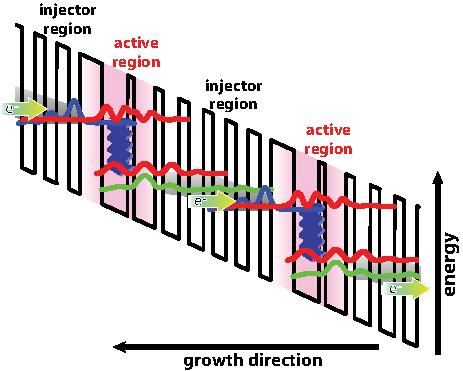
\includegraphics[width=5.25in]{introduction/qcl}
\caption[Basic QC laser band diagram]{\tn{\textbf{Basic QC laser band diagram.}}  The conduction band edge of the alternating wide and narrow bandgap materials are is shown, along with the stationary wavefunctions of the quantum wells.  QC lasers have an active region, where optical transitions are engineered to occur, and an injector region, which stitches together successively ``cascaded'' active regions.  When a sufficient electric field is applied, indicated in the figure by the constant slope, electrons are able to transit through the entire QC structure.}
\label{intro:pictorial_qcl}
\end{figure}

A QC laser's design can be divided into two sections: the active regions and the injector regions.  QC active regions have at least three important energy ``states,'' which are in fact energy sub-bands. Two states are needed to form the upper and lower energy states of the optical transition.  The positions of these states are selected to give an energy separation of the desired photon energy, and they are usually designed to have large overlap integrals to yield a large oscillator strength.  A third important active region state is placed below the lower laser state; an energy separation of at least one longitudinal optical (LO) phonon is used.  LO phonons represent the fastest electron scattering mechanism in semiconductors.  This lowest energy state is thus intended to quickly empty the lower energy level, and hence for the first two states provide an in-built population inversion.

The other important QC laser section is the QC injector region.  QC injectors do all of the important functions necessary to ``stitch together'' consecutive active regions.  That is, QC injectors impart the ability to take electrons from the lower states in one active region and inject them into the upper laser state of the next, down-stream active region.  Through this stitching together of multiple active--injector region periods, multiple photons are emitted for each single electron that passes through the structure.  A detailed examination of the role of injector regions is given in Chapter 5.

%Unipolar devices.  The device is entirely n-doped.  Everything happens in the conduction band.  So it's intersubband.  When showing band diagrams, completely ignore the valence band.  Only show the conduction band.




%
%
%\subsection{Current Capabilities}
%
%Wavelength range: 4.2 � 12 �m
%
%Wall-plug efficiency: ? 20 %
%
%usually << 20%
%
%Single spectral mode, single spatial mode
%
%Low-input power, low-output power devices
%
%Long operating lifetimes
%
%They�re light weight!
%
%
%
%\subsection{Current Challenges}




\section{The QC Development Process}

The process of producing QC laser can be divided into three basic steps: design, growth, and fabrication.  Each represents a critically important skill set, and high performance QC laser production requires high quality in all three areas.

\subsection{Design}

\begin{figure}[tp]
\centering
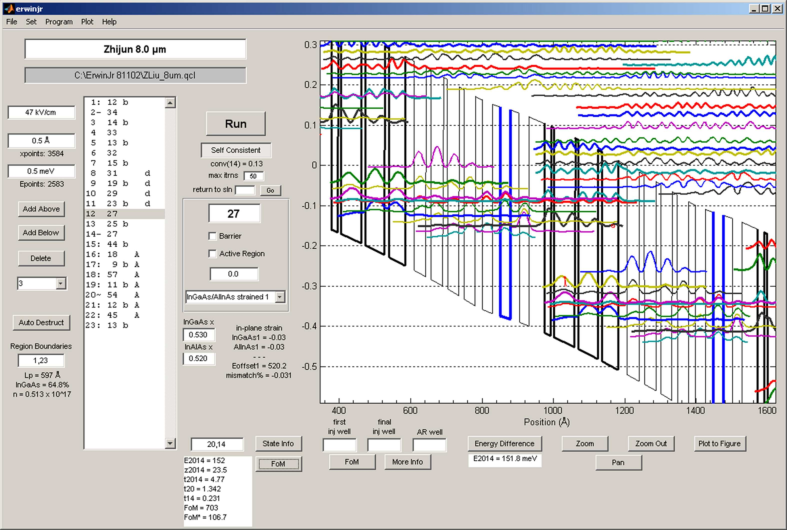
\includegraphics[width=6in]{introduction/erwinjr}
\caption[ErwinJr QC laser design software]{\tn{\textbf{ErwinJr QC laser design software.}}  QC laser design has been aided by advances in design tools.}
\label{chpt1:shooting_example}
\end{figure}

QC laser design is the first step of laser development.  The high degree of flexibility afforded by the QC concept makes design both a creative and challenging process.  Successful QC designs have indeed been quite varied in architecture.  For example, after years of following the single LO phonon active region convention, Beck \emph{et al.} realized superior performance by using two stacked LO phonon transitions in the active region to empty the lower laser state \cite{Beck:Science:2002}.  A superlattice QC structure, first demonstrated in 1997 \cite{Scamarcio:Science:1997:superlattice}, creates dense ``minibands'' of states by using much narrower well and barrier layers as compared to conventional QC structures.  Both Raman lasers \cite{Troccoli:Nature:2005} and Bloch gain \cite{Terazzi:NPhys:2007} have been demonstrated in QC structures.  The list of creative design architectures goes on and on.  Clearly, the flexibility is advantageous for capitalizing on the discovery of new physical phenomena and for implementing new design strategies.

QC laser design is accomplished using a set of tools that primarily function by solving the Schr\"{o}dinger equation.  Figure~\ref{chpt1:shooting_example} shows a screen shot of our recently developed software ErwinJr, which can solve for the energy states of complex and large QC structures in a matter of seconds.  This ability rapidly speeds the QC design process.

\subsection{Growth}

The epitaxial growth of QC lasers is accomplished either by molecular beam epitaxy (MBE) or metal-organic vapor phase deposition (MOVPE or MOCVD).  Both growth methods are highly automated processes, where computers are used to control deposition rates and times.  Such automation is absolutely necessary due to the extreme complexity of QC structures.  The growth of the hundreds of individual layers required for QC structures by more manual processes (such as liquid phase epitaxy, for example) would simply be prohibitive.  Excellent reviews of both growth methods can be found in the \emph{Proceedings of the IEEE}: Ref.~\cite{Cheng:ProcIEEE:1997} for MBE and Ref.~\cite{Coleman:ProcIEEE:1997:MOCVD} for MOVPE.

\subsection{Fabrication}

Methods of QC laser fabrication have become much more advanced since the initial QC laser reported in 1994.  The two primary concerns for laser fabrication are creating a low optical loss waveguide and creating a path for heat to rapidly leave the QC active core.  The four basic processing methods used in this thesis are described below.

The most basic processing method is the ridge laser, shown in Fig.~\ref{chpt1:fab_a}.  The ridge laser is the fastest to process, but also has the least capable heat extraction capabilities.  It is best suited for rapid testing of QC laser material, especially applicable when a comparison among the performance of multiple QC structures is needed.

A more advanced processing method is the double trench, as shown in Fig.~\ref{chpt1:fab_b}.  These laser structures are especially able to capitalize on using thick ($\sim\!5$~\um) Au as the top contact, which provides a rapid thermal transport path out of the active region.  Double trench lasers have shown the capability of room temperature, continuous wave performance \cite{Liu:PTL:2006}.

\begin{figure}[tp]%
\centering%
%\vspace{0.26in}%
\subfloat[]{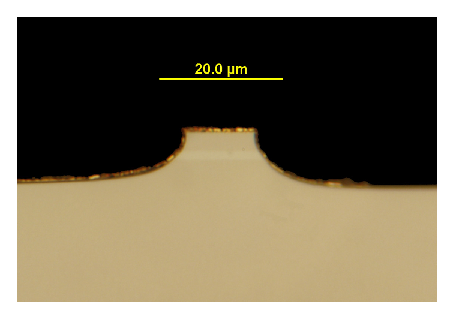
\includegraphics[width=2.8in]{introduction/proc_ridge_eps}%
\label{chpt1:fab_a}}%
\hfil%
\subfloat[]{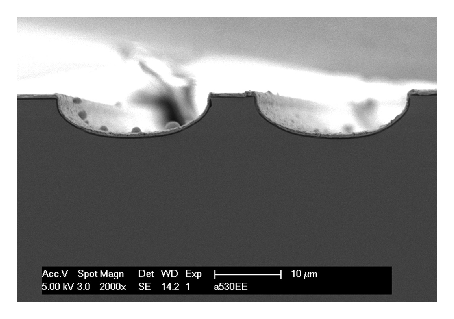
\includegraphics[width=2.8in]{introduction/proc_dt_eps}%
\label{chpt1:fab_b}}%
\\%
\subfloat[]{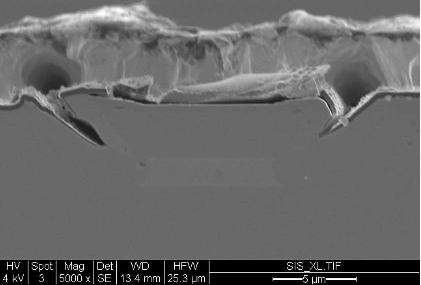
\includegraphics[width=2.8in]{introduction/proc_bh_eps}%
\label{chpt1:fab_c}}%
\hfil%
\subfloat[]{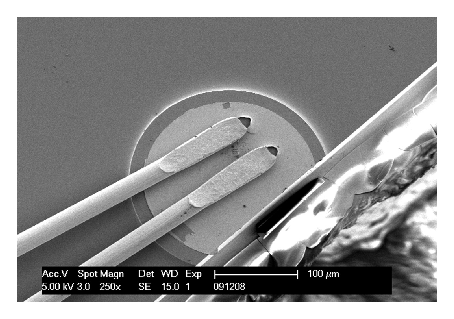
\includegraphics[width=2.8in]{introduction/proc_EL_eps}%
\label{chpt1:fab_d}}%
\caption[QC laser fabrication methods]{\tn{\textbf{QC laser fabrication methods.}}   Ridge lasers, as shown in \tn{(a)}, are the most basic laser type and are the most straight-forward and fast to process.  More complex structures, such as the double trench ridge in \tn{(b)}, are more difficult to process but can have improved heat extraction capabilities.  Buried heterostructures, shown in \tn{(c)}, are the most advanced and highest performing structures; they are also the most complicated to fabricate, as they require a second InP growth step. Electroluminescence mesas, as shown in \tn{(d)}, are used for QC structure characterization.  They have the particular advantage of suppressing optical feedback and therefore suppressing lasing.}
\label{chpt1:fab}
\end{figure}

The most advanced, highest performing, and time-intensive processing method is the buried heterostructure (BH), shown in Fig.~\ref{chpt1:fab_c}.  These structures were the first to demonstrated room temperature, continuous wave performance \cite{Beck:Science:2002}.  Improved packaging technologies, such as mounting lasers epitaxial-side down on diamond heat sinks \cite{Razeghi:SPIE:2009}, have also shown dramatic performance improvements.

The electroluminescence (EL) mesa, as shown in Fig.~\ref{chpt1:fab_d}, is another type of QC structure that is most often used for test and analysis purposes.  These structures are specifically designed to suppress optical feedback, so that emission is purely from spontaneous emission.

\section{Thesis Overview}

This thesis seeks to demonstrate the power of the quantum cascade as a flexible device technology platform.  Never before has a laser system afforded engineers so much control over its fundamental, internal mechanisms.  Truly, the QC concept imparts the unprecedented ability to create new device architectures that incorporate new operation concepts.  Throughout this thesis, we provide examples of how this flexibility can be exploited to improve device performance and expand device capabilities.  %Such as Excited state and Short Injector lasers.  k-space lasing.  And within many different materials systems: ii-vi.

In Chapter 2, we provide a theoretical foundation for basic operation principles of QC lasers.  Key tools used in laser design, such as accurate solutions to the Schr\"odinger equation and  the optical dipole matrix element, are explicitly discussed.  Derivations for important device performance parameters, such as threshold current and wall-plug efficiency, are given with sufficient detail to clearly understand the origins and contributions of important design parameters.

As an example of the flexibility of the technology platform, Chapter 3 discusses implementing QC structures in an entirely new materials system: ZnCdSe / ZnCdMgSe \cite{Franz:APL:2008}.  This II--VI materials system has some properties that may be advantageous over the currently used III--V materials system, such as larger conduction band offsets, which ultimately may be useful for developing shorter wavelength QC lasers than those currently available.

In contrast, the motivation for Chapter 4 starts with expanding the capabilities of QC lasers on the long wavelength side.  Here, we present a new QC architecture---one which employs optical transitions made completely of quantum well excited states \cite{Franz:APL:2007}.  These excited state structures have the ability to compensate for many of the deleterious factors that make long-wavelength lasing so difficult.  Through experimenting with this new structure, we found the unexpected and unique property of lasing high in \emph{k}-space \cite{Franz:NPhoton:2009}.

Chapter 5 presents a fundamental re-examination of the role of QC injector regions.  Since the injector regions are not the source of photons, they can in some ways be viewed as ``wasted space.''  However, injector regions practically serve several functions that are crucial to high laser performance.  Here, we look at minimizing injector length, and we employ QC designs that drastically reduce the overall period length of the structure.  Like in the results of Chapter 4, we observe unique and unexpected properties.  These observations allow us to draw new insights into and understanding of fundamental QC laser operation mechanisms.

Finally, concluding remarks are given in Chapter 6, along with an outlook for the future of QC technology.

%Explain why field can move so rapidly.  Quantum cascade concept accommodates new design architectures.


%
%\bibliographystyle{kale3}
%\bibliography{biblio}
%\end{document} 